\subsection{Rekonstruksi Citra}
% Selain dapat digunakan dalam minimalisasi fungsi, skema iterasi Sabri juga dapat digunakan dalam permasalahan \textit{split feasibility}, yang memiliki aplikasi nyata dalam rekonstruksi citra.
Dalam rekonstruksi citra, skema iterasi dapat dipandang sebagai alat untuk menyelesaikan permasalahan \textit{split feasibility}. Permasalahan \textit{split feasibility} ini dikenalkan oleh Censor dan Elfving pada tahun 1994, yang diformulasikan sebagai 
\begin{align}\label{eq:sfp}
    \text{Cari titik } x^*\in C \quad \text{yang memenuhi}\quad Ax^*\in Q,
\end{align}
dengan $C$ dan $Q$ berturut-turut adalah himpunan bagian tertutup dan konveks dari ruang Hilbert $H_1$ dan $H_2$, serta $A:H_1\to H_2$ adalah transformasi linier terbatas \cite{Censor1994}. Permasalahan \eqref{eq:sfp} disebut konsisten jika setidaknya memiliki satu solusi. Suatu titik $x^*\in C$ merupakan solusi dari permasalahan tersebut jika dan hanya jika $x^*$ memenuhi persamaan titik tetap 
\begin{align}
    x=P_C(I-\gamma A^*(I-P_Q)A)x,
\end{align}
dengan $P_C$ dan $P_Q$ adalah proyeksi titik terdekat pada $C$ dan $Q$, secara berturut-turut, $\gamma>0$, dan $A^*$ adalah transformasi adjoin dari $A$ \cite{feng2019}. Dalam hal ini parameter $\gamma$ dipilih sehingga $0<\gamma<\frac{2}{k}$ dengan $k$ adalah radius spektral dari $A^*A$, yaitu 
nilai maksimum dari mutlak nilai eigen dari $A^*A$.
Kemudian, berdasarkan Contoh \ref{con:hilbert}, diketahui bahwa ruang Hilbert merupakan ruang $CAT(0)$ yang juga merupakan ruang $CAT_p(0)$ dengan $p=2$. Selanjutnya, berdasarkan hasil dari Byrne \cite{Byrne2003}, pemetaan $T:C\to C$ yang didefinisikan sebagai $T(x)=P_C(I-\gamma A^*(I-P_Q)A)x$ adalah pemetaan nonekspansif. Oleh karena itu, pemetaan ini juga merupakan pemetaan $(\alpha,\beta,\gamma)$-nonekspansif.

Dari permasalahan tersebut, skema iterasi Sabri dapat digunakan sebagaimana Teorema berikut.
\begin{thm}
    Diberikan ruang Hilbert $H$ yang kompak dan $C$ adalah himpunan bagian yang tertutup dan konveks dari $H$.
    Jika permasalahan \eqref{eq:sfp} konsisten dengan solusi yang tunggal dan $\gamma\in (0,\frac{2}{k})$ dengan $k$ adalah radius spektral dari $A^*A$, maka pemetaan $T:C\to C$ yang didefinisikan sebagai $$T(x)=P_C(I-\gamma A^*(I-P_Q)A)x$$ 
    merupakan pemetaan $(\alpha,\beta,\gamma)$-nonekspansif, serta barisan $\{x_n\}$ yang didefinisikan sebagai
    \begin{flalign}
        \begin{cases}
            q_n &= T\qty((1-c_n)x_n\oplus c_n T(x_n)) \\
            y_n &= T(T(q_n)) \\
            x_{n+1} &= T\qty((1-a_n)T(q_n)\oplus a_n T(y_n)) 
        \end{cases}, 
    \end{flalign}
    dengan $\{a_n\},\{c_n\}\subseteq [a,b]\subset (0,1)$ konvergen kuat ke solusi tunggal $x^*\in C$ dari permasalahan \eqref{eq:sfp} untuk setiap nilai awal $x_0\in C$.
    \begin{bukti}
        Berdasarkan hasil dari Byrne (lihat \cite{Byrne2003}), diperoleh bahwa pemetaan $T$ yang memenuhi kondisi tersebut adalah pemetaan nonekspansif sehingga juga merupakan $(\alpha,\beta,\gamma)$-nonekpansif. Kemudian, berdasarkan Contoh \ref{con:lpcatp}, didapatkan bahwa $H$ adalah ruang $CAT(0)$ yang juga merupakan ruang $CAT_p(0)$ dengan $p=2$. Akibatnya, dengan Teorema \ref{thm:konvK}, diperoleh bahwa $\{x_n\}$ konvergen kuat ke titik tetap dari $T$, yang berarti $\{x_n\}$ konvergen kuat ke solusi tunggal dari $x^*\in C$.
    \end{bukti}
\end{thm}

Hasil ini dapat diterapkan pada permasalahan rekonstruksi citra tomografi. Permasalahan tersebut memiliki peranan penting dalam dunia medis, khususnya dalam rekonstruksi citra dari \textit{CT-Scan}, yang datanya berupa proyeksi yang dikenal sebagai sinogram. Pada umumnya, rekonstruksi citra organ tubuh dari data sinogram dilakukan menggunakan proyeksi mundur berfilter (\textit{filtered back projection}). Dari segi waktu komputasi, metode ini relatif cepat dalam menghasilkan citra. Namun, metode tersebut memiliki keterbatasan dalam kualitas citra yang dihasilkan, akibat tingginya tingkat derau. Untuk mereduksi derau pada citra hasil rekonstruksi, metode ini memerlukan dosis radiasi yang lebih tinggi pada pasien, yang berpotensi menimbulkan dampak negatif pada kesehatan pasien. Sebagai alternatif, rekonstruksi citra dapat dilakukan menggunakan proyeksi mundur tanpa filter yang dikombinasikan dengan algoritma skema iterasi. Pendekatan ini terbukti mampu mereduksi derau secara signifikan, yaitu sekitar 40\% sampai 70\% dibandingkan dengan metode proyeksi mundur berfilter \cite{Ramage2023}. 


Pada bagian ini, dilakukan simulasi rekonstruksi citra tomografi berbasis skema iterasi Sabri. Transformasi maju $A$ yang digunakan adalah transformasi Radon, sedangkan himpunan batas $C$ dan $Q$ adalah himpunan bagian yang konveks dari suatu ruang Euclid $\mathbb{R}^n$, yang masing-masing merepresentasikan solusi \textit{feasible} untuk citra dan domain proyeksi. 

Berikut ini diberikan gambaran bagaimana skema iterasi Sabri dapat diterapkan dalam rekonstruksi citra tomografi di ruang $CAT_p(0)$.
\begin{figure}[H]
    \label{fig:sinorekon}
    \centering
    \tikzstyle{startstop} = [ellipse, 
minimum width=3cm, 
minimum height=0.5cm,
text centered, 
draw=black]

\tikzstyle{io} = [trapezium, 
trapezium stretches=true, % A later addition
trapezium left angle=70, 
trapezium right angle=110, 
minimum width=6cm, 
minimum height=0.5cm, text centered, 
draw=black]

\tikzstyle{process} = [rectangle, 
minimum height=0.5cm, 
text centered, 
text width=4cm, 
draw=black]

\tikzstyle{decision} = [diamond, 
minimum width=2cm, 
minimum height=0.5cm, 
text centered, 
aspect=1.8,
inner sep=2pt,
draw=black]
\tikzstyle{arrow} = [thick,->,>=stealth]
\begin{tikzpicture}[scale=1.2,node distance=1.8cm]

\node (sino) [startstop]
{Data Sinogram};

\node (data2d) [process, below left of=sino, xshift=-2cm,yshift=-0.7cm]
{Data 2D};

\node (data3d) [process, below right of=sino, xshift=2cm]
{Data 3D};

% \node (vec2d) [process, below of=data2d]
% {Vektorisasi\\
% data 2D};

\node (slice) [process, below of=data3d]
{\textit{Slice} menjadi\\
potongan 2D};

\node (rn) [startstop, below of=sino, yshift=-3.5cm, align=center]
{Vektor data $\mathbb{R}^n$\\
(Ruang Euclid)};

\draw [arrow] (sino) -- (data2d);
\draw [arrow] (sino) -- (data3d);

% \draw [arrow] (data2d) -- (vec2d);
\draw [arrow] (data3d) -- (slice);

\draw [arrow] (data2d.south) |- (rn.west);
\draw [arrow] (slice.south) |- (rn.east);

\end{tikzpicture}
    \caption{\centering Diagram Data Sinogram ke Ruang Euclid dalam Rekonstruksi Citra}
\end{figure}
\begin{figure}[H]
    \label{fig:himp}
\centering
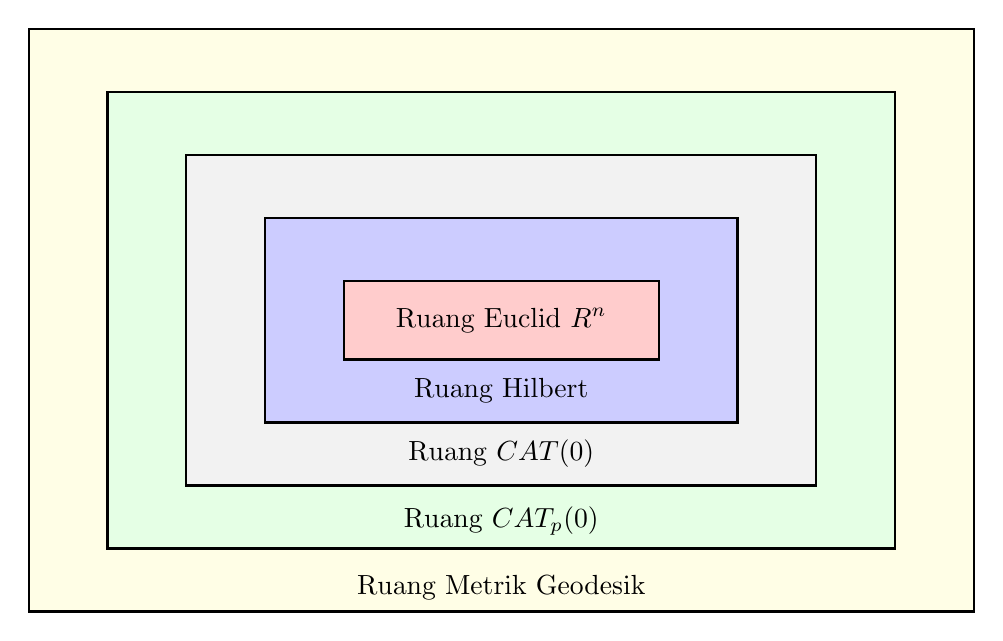
\begin{tikzpicture}[scale=1, every node/.style={transform shape}]


\draw[thick,fill=yellow!10] (-6,-3.7) rectangle (6,3.7);
\node at (0,-3.4) {Ruang Metrik Geodesik};

\draw[thick,fill=green!10] (-5,-2.9) rectangle (5,2.9);
\node at (0,-2.55) {Ruang $CAT_p(0)$};

\draw[thick, fill=gray!10] (-4,-2.1) rectangle (4,2.1);
\node at (0,-1.7) {Ruang $CAT(0)$};

\draw[thick, fill=blue!20] (-3,-1.3) rectangle (3,1.3);
\node at (0,-0.9) {Ruang Hilbert};

\draw[thick,fill=red!20] (-2,-0.5) rectangle (2,0.5);
\node at (0,0) {Ruang Euclid $\mathbb{R}^n$};


\end{tikzpicture}
\caption{\centering Hubungan ruang Euclid, Hilbert, $CAT(0)$, $CAT_p(0)$, dan ruang metrik geodesik}
\end{figure}






Pada simulasi ini, digunakan bahasa pemrograman Python dengan bantuan pustaka Scikit-image. Data citra yang digunakan adalah Shepp-Logan Phantom $x^*\in \mathbb{R}^n$ dengan resolusi $512\times 512$. Shepp-Logan Phantom dipilih karena merupakan model sintetik yang dirancang untuk menyerupai potongan gambar bagian dalam kepala manusia, sehingga sering digunakan dalam penelitian tomografi untuk menguji kemampuan algoritma rekonstruksi dalam membedakan struktur dengan tingkat kontras yang berbeda. Selanjutnya, data sinogram dibentuk sebagai $Q=Ax^*$ dengan menerapkan transformasi Radon pada sudut-sudut proyeksi yang terdistribusi merata pada interval $[0,180^{\circ})$. Tujuan simulasi ini adalah merekonstruksi citra $x^*$ berdasarkan data sinogram tersebut menggunakan skema iterasi Sabri. Untuk itu, digunakan pemetaan 
\begin{align}\label{eq:rekonoperator}
    T(x)=P_C(x-\gamma A^*(Ax-Q)),
\end{align}
dengan $A^*$ merupakan aproksimasi dari transformasi adjoin $A$ yang diperoleh menggunakan proyeksi mundur tanpa filter, serta $P_C$ menyatakan operator proyeksi ke himpunan batas $C=[0,1]^n$. 

Pada \ref{fig:flowrekonstruksi} diberikan diagram alir dari skema iterasi Sabri yang digunakan dalam simulasi rekonstruksi citra tomografi dengan parameter-parameter yang digunakan disajikan pada \ref{tab:parametersim}.
\begin{figure}[H]
    \centering
    \tikzstyle{startstop} = [ellipse, 
minimum width=5.5cm, 
minimum height=0.5cm,
text centered, 
draw=black]

\tikzstyle{io} = [trapezium, 
trapezium stretches=true, % A later addition
trapezium left angle=70, 
trapezium right angle=110, 
minimum width=6cm, 
minimum height=0.5cm, text centered, 
draw=black]

\tikzstyle{process} = [rectangle, 
minimum height=0.5cm, 
text centered, 
text width=8.5cm, 
draw=black]

\tikzstyle{decision} = [diamond, 
minimum width=2cm, 
minimum height=0.5cm, 
text centered, 
aspect=1.8,
inner sep=2pt,
draw=black]
\tikzstyle{arrow} = [thick,->,>=stealth]

\begin{tikzpicture}[node distance=1.4cm,scale=1, every node/.style={transform shape}]

% ===== Nodes =====
\node (start) [startstop] 
{Mulai};

\node (input) [io, below of=start,align=center,yshift=-0.3cm] 
    {Inisialisasi data Sinogram $Q$, gambar awal $x_0\in \mathbb{R}^n$,\\
     $k=0$, batas iterasi $K$, dan parameter $\gamma$, $\{a_k\},\{c_k\}\subseteq (0,1)$};

\node (hitung) [process, below of=input,yshift=-0.3cm] 
{Definisikan $T(x)$ sesuai persamaan \eqref{eq:rekonoperator}};

\node (qn) [process, below of=hitung] 
{$q_k = T\big((1-c_k)x_k + c_k T x_k\big)$};

\node (yn) [process, below of=qn] 
{$y_k = T(Tq_k)$};

\node (xn) [process, below of=yn] 
{$x_{k+1} = T\big((1-a_k)Tq_k + a_k Ty_k\big)$};

\node (decision) [decision, below of=xn, yshift=-0.8cm,align=center] 
{Apakah\\$k\geq K$?};

\node (stop) [startstop, below of=decision, yshift=-0.8cm] 
{Selesai};

% ===== Arrows =====
\draw [arrow] (start) -- (input);
\draw [arrow] (input) -- (hitung);
\draw [arrow] (hitung) -- (qn);
\draw [arrow] (qn) -- (yn);
\draw [arrow] (yn) -- (xn);
\draw [arrow] (xn) -- (decision);
\draw [arrow] (decision) -- node[anchor=east]{Ya} (stop);

\draw [arrow] (decision.east) -- ++(4,0) 
node[anchor=west]{Tidak}
|- (qn.east);

\end{tikzpicture}

    \caption{\centering Diagram alir skema iterasi Sabri untuk rekonstruksi citra tomografi}
    \label{fig:flowrekonstruksi}
\end{figure}


\begin{table}[H]
    \centering
    \caption{Parameter simulasi rekonstruksi citra}
    \begin{tabular}{ll}
    \hline
    \textbf{Parameter} & \textbf{Nilai/Deskripsi}\\
    \hline
    Ukuran gambar     &  $512\times 512$ \\
    Sudut proyeksi     &  180 terdistribusi merata pada $[0^\circ, 180^\circ)$\\
    Transformasi maju $A$ & Transformasi Radon\\
    Transformasi adjoin $A^*$ & Proyeksi mundur tanpa filter\\
    Himpunan batas $C$ & $[0,1]^n$\\
    Nilai awal $x_0$ & $x_0=\mathbf{0}$\\
    Jumlah iterasi & 480\\
    Parameter $\gamma$ & Konstan: 0.002447\\
    Parameter $a_n,c_n$ & Konstan: $a_n=0.42, c_n=0.31$\\
    Implementasi & Google Colab dengan scikit-image, matplotlib\\
    \hline
    \end{tabular}
    \label{tab:parametersim}
\end{table}

Data awal dari simulasi tersebut disajikan pada \ref{fig:rekoncit}. Kemudian hasil simulasi dari rekonstruksi citra tersebut pada iterasi ke-5, 10, 30, 60, 90, 120, 240, dan 480 diberikan oleh \ref{fig:rekoncit2} dan \ref{fig:rekoncit3}. Pada iterasi ke-5, terlihat bahwa derau dari citra tersebut masih cukup tinggi, yang juga tertera pada nilai (\textit{peak signal noise ratio}) PSNR, yaitu 22.55 dB. Nilai PSNR dari citra tersebut juga makin membesar pada iterasi ke-10 dan 30, hingga iterasi ke-480, dengan nilai PSNR citra tersebut adalah 40.73 dB, yang mengindikasikan semakin sedikit derau pada citra. Waktu yang diperlukan dalam simulasi rekonstruksi citra ini adalah 11024.39 detik.
\begin{figure}[H]
    \centering
    \includegraphics[width=0.95\linewidth]{Bab_4/citrafix.png}
    \caption{Data awal sinogram dan citra asli}
    \label{fig:rekoncit}
\end{figure}
\begin{figure}[H]
    \centering
    \includegraphics[width=0.95\linewidth]{Bab_4/citrafixx2.png}
    \caption{Hasil rekonstruksi citra pada iterasi ke-5 dan 10}
    \label{fig:rekoncit2}
\end{figure}
\newpage
\begin{figure}[H]
        \centering
    \includegraphics[width=0.95\linewidth]{Bab_4/citrafixx3.png}
    \caption{Hasil rekonstruksi citra pada iterasi ke-30, 60, 90, 120, 240, dan 480}
    \label{fig:rekoncit3}
\end{figure}
\newpage
Pada \ref{fig:galatrek} dan Lampiran \ref{lamp:mse}, diberikan grafik dan tabel nilai dari metrik PSNR dan MSE dari citra hasil rekonstruksi pada tiap iterasinya. Terlihat bahwa nilai galat, yaitu (\textit{mean squared error}) dari citra tersebut relatif kecil pada iterasi ke-480, yaitu $8\times 10^{-5}$, dibandingkan dengan galat pada iterasi pertama, yaitu $2\times 10^{-2}$. Terlihat pula bahwa nilai metrik PSNR dan MSE tersebut berturut-turut naik dan turun pada tiap iterasinya, sesuai dengan peningkatan kualitas citra pada \ref{fig:rekoncit2} dan \ref{fig:rekoncit3}, yang menunjukkan bahwa skema iterasi Sabri dapat digunakan dalam rekonstruksi citra tomografi.
\begin{figure}[H]
    \centering
    \includegraphics[width=\linewidth]{Bab_4/galatrek.png}
    \caption{Metrik PSNR dan MSE dari rekonstruksi citra}
    \label{fig:galatrek}
\end{figure}
